\documentclass[a4paper, 12pt]{article}
\usepackage{graphicx}
\usepackage{enumitem}
\usepackage{mathtools}
\usepackage{hyperref}
\usepackage{caption}
\usepackage{subcaption}
\def\code#1{\texttt{#1}}
\def\f#1{Figure \ref{fig:#1}}
\begin{document}

\title{\vspace{4.0cm}Applied GPU Programming - Assignment III\\
\large DD2360 HT20}
\author{Pontus Asp}
\date{\today}
\maketitle
\thispagestyle{empty}
\pagenumbering{roman}
\newpage

\clearpage
\pagenumbering{arabic}

% Write here ->
\section{Git repository}
I uploaded my git repository to GitHub. I use the same git repository for the entire course but the folder structure requested is still followed under the root folder. I also have 2 extra directories, one for this report and one where I have code from tutorials.
\\\\
Here is the link to my git repository:\\
\url{https://github.com/pontusasp/kth-dd2360/tree/master/Assignment_3}


% 1. Explain how the mapping of GPU thread and thread blocks (which is already implemented for you in the code) is working.

% 2. Explain why shared memory can (theoretically) improve performance.

% 3. Explain why the resulting image looks like a "grid" when the kernel is simply copying in pixels to the shared block. Explain how this is solved and what are the cases.

% 4. There are several images of different sizes in the image folder. Try running the program on them and report how their execution time relates to file sizes.
\section{Exercise 1}



% 1. What are the differences between pageable memory and pinned memory, what are the tradeoffs?

% 2. Do you see any difference in terms of break down of execution time after changing to pinned memory from pageable memory?

% 3. What is a managed memory? What are the implications of using managed memory?

% 4. If you are using Tegner or lab computers, the use of managed memory will result in an implicit memory copy before CUDA kernel launch. Why is that?
\section{Exercise 2}


% 1. What are the advantages of using CUDA streams and asynchronous memory copies?

% 2. What is the performance improvement (if any) in using more than one CUDA stream?

% 3. What is the impact of batch size on the performance?
\section{Exercise 3}


% 1. Explain why is the matrix size has to be a multiple of 16?

% 2. Refer to shared_sgemm_kernel(). There are two __syncthreads() in the loop. What are they used for, in the context of this code?
%
%       2.1. What is the directive that can potentially improve performance in the actual multiplication? What does it do?
%
%       2.2. There is a large speedup after switching from using global memory to shared memory, compared to the Edge Detector in Exercise 1. What might be the reason?

% 3. Refer to cublas_sgemm(). We asked that you compute LaTeX: C\:=BAC = B A instead of LaTeX: C=ABC = A B. It has to do with an important property of cuBLAS. What is that, and why do we do LaTeX: C\:=BAC = B A?

% 4. Run the program with different input sizes, for example from 64, 128, ... , to 4096. Make a grouped bar plot of the execution times of the different versions (CPU, GPU Global, GPU Shared, GPU cuBLAS). You can plot CPU results in a separate figure if the execution time goes out of the scale comparing to the rest.

% 5. The way the execution time benchmark that is implemented in the code is good enough for this exercise, but in general it is not a good way to do a benchmark. Why?
\section{Bonus Exercise}



% Write here <--

\end{document}



%\begin{figure}
%  \centering
%  \begin{subfigure}{.5\textwidth}
%    \centering
%    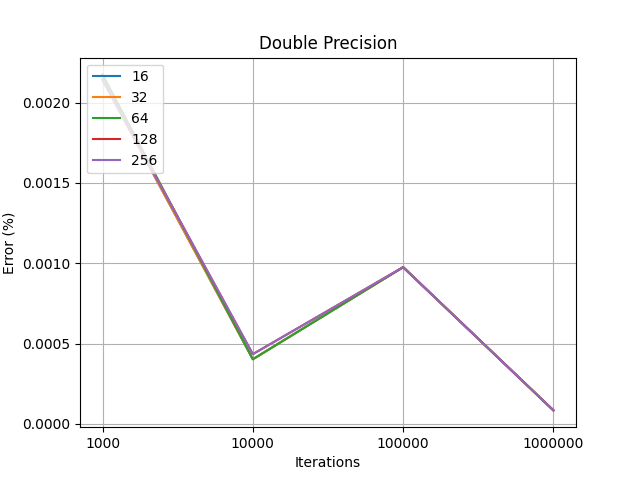
\includegraphics[width=1\linewidth]{graphs/ex_bonus_double_error.png}
%    \caption{Double Precision}
%    \label{fig:ex-single-double-error}
%  \end{subfigure}%
%  \begin{subfigure}{.5\textwidth}
%    \centering
%    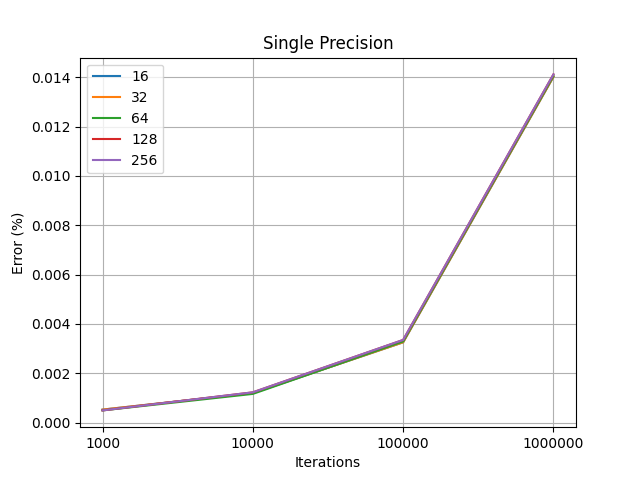
\includegraphics[width=1\linewidth]{graphs/ex_bonus_single_error.png}
%    \caption{Single Precision}
%    \label{fig:ex-bonus-single-error}
%  \end{subfigure}
%  \caption{Graphs of error using double and single precision with different amounts of iterations and block sizes.}
%  \label{fig:fig:ex-bonus-error}
%\end{figure}